\documentclass{report}
\usepackage{lmodern}
\author{Andreas Schachner}
\title{Dokumentation zum Uni-Heidelberg-App-Projekt}
\usepackage[top=3cm, bottom=3cm, inner=3.5cm, outer=3cm]{geometry}
\usepackage[T1]{fontenc}
\usepackage{amssymb}
\usepackage{pifont} 
\usepackage{longtable} 
\usepackage{tabularx} 
\usepackage{graphicx} 
\usepackage{amsmath}
\usepackage[ngerman]{babel} 
\usepackage[automark,headsepline,plainheadsepline]{scrpage2}
\usepackage{endnotes}
\usepackage{csquotes}
\usepackage{hyperref}
\hypersetup{colorlinks=true,urlcolor=blue,linkcolor=blue}
\usepackage{relsize}
\usepackage{xcolor}
\usepackage{soul}
\usepackage{endnotes}
\setcounter{tocdepth}{2}
\pagestyle{scrheadings}
\ihead[\rightmark]{\rightmark} \chead[\pagemark]{}
\usepackage{pst-all}
\usepackage{blindtext}
\usepackage{fontspec}
\newfontfamily{\codefont}{Menlo}

\usepackage{color,xcolor}
\definecolor{nsclass}{RGB}{124,32,176}
\definecolor{atnotation}{RGB}{204,0,164}
\definecolor{import}{RGB}{128,70,30}
\definecolor{comment}{RGB}{0,140,0}
\definecolor{string}{RGB}{229,0,0}
\definecolor{method}{RGB}{70,0,134}
\definecolor{class}{RGB}{59,131,138}
\definecolor{custommethod}{RGB}{32,90,95}
\definecolor{number}{RGB}{56,0,225}
\definecolor{customgray}{RGB}{211,211,211}
\definecolor{highlight}{RGB}{255,243,153}

\usepackage{listings}
\lstloadlanguages{[Objective]C,bash}
\lstset{language=[Objective]C,tabsize=4, keepspaces=false,
    xleftmargin=0em,xrightmargin=-1em, aboveskip=1em, % Margin adjustment
    %backgroundcolor=\color{customgray},    % Background color (Default:gray)
    frame=none,                            % Frame not needed
    breakindent=22pt,
    numbers=left,stepnumber=1,numberstyle=\tiny\color{black}\codefont,
    basicstyle=\fontsize{9pt}{1em}\selectfont\codefont,
    commentstyle=\fontsize{9pt}{0.75em}\selectfont\codefont\color{comment},
    showspaces=false,
    showstringspaces=false,
    flexiblecolumns=true,
    breaklines=true, breakautoindent=true,breakindent=4em,
    escapeinside={/*@}{@*/},
    morecomment=[s][\color{string}]{@"}{"},
    morecomment=[l][\color{import}]{\#},
    morecomment=**[s][\color{nsclass}]{NS}{];},
    morecomment=**[s][\color{nsclass}]{UI}{];},
    morecomment=**[s][\color{nsclass}]{NS}{(},
    morecomment=**[s][\color{nsclass}]{UI}{)},
    morecomment=**[s][\color{nsclass}]{UI}{*},
    morecomment=**[s][\color{nsclass}]{NS}{*},
    morecomment=*[s][\color{nsclass}]{UI}{\ },
    morecomment=*[s][\color{nsclass}]{NS}{\ },
    literate= {Ö}{{\"O}}1 {Ä}{{\"A}}1 {Ü}{{\"U}}1 {ß}{{\ss}}2 {ü}{{\"u}}1
 {ä}{{\"a}}1 {ö}{{\"o}}1,
}
\lstset{emph=[1]{  % <--Add your own Class Names before the percentage mark
       },emphstyle=[1]{\color{class}},
       moreemph=[5]{ % <--Add your own Method Names before the percentage mark
       },emphstyle=[5]{\color{method}},
}
\lstset{
    emph=[3]{@implementation, @synthesize, @interface, @property, @dynamic,
    @end, @protocol, @class, @selector, break, case, catch, class, copy, const, __finally, __exception,
    __try, const_cast, continue, private, public, protected, __declspec,
    default, delete, deprecated, dllexport, dllimport, do, dynamic_cast, else,
    enum, explicit, extern, if, for, friend, getter, goto, inline, mutable,
    naked, namespace, new, nil, NO, noinline, nonatomic, noreturn, nothrow,
    NULL, readonly, readwrite, register, reinterpret_cast, retain, return,
    SEL, selectany, self, setter, sizeof, static, static_cast, strong, struct, super,
    switch, template, thread, throw, true, false, try, typedef, typeid,
    typename, union, using, uuid, virtual, void, volatile, weak, whcar_t, while, YES,
    ATOM, BOOL, BOOLEAN, BYTE, CHAR, COLORREF, DWORD, DWORDLONG, DWORD_PTR,
    DWORD32,DWORD64, FLOAT, HACCEL, HALF_PTR, HANDLE, HBITMAP, HBRUSH,
    HCOLORSPACE, HCONV, HCONVLIST, HCURSOR, HDC, HDDEDATA, HDESK, HDROP,
    HDWP, HENHMETAFILE, HFILE, HFONT, HGDIOBJ, HGLOBAL, HHOOK, HICON,
    HINSTANCE, HKEY, HKL, HLOCAL, HMENU, HMETAFILE, HMODULE, HMONITOR,
    HPALETTE, HPEN, HRESULT, HRGN, HRSRC, HSZ, HWINSTA, HWND, INT, INT_PTR,
    INT32, INT64, LANGID, LCID, LCTYPE, LGRPID, LONG, LONGLONG, LONG_PTR,
    LONG32, LONG64, LPARAM, LPBOOL, LPBYTE, LPCOLORREF, LPCSTR, LPCTSTR,
    LPCVOID, LPCWSTR, LPDWORD, LPHANDLE, LPINT, LPLONG, LPSTR, LPTSTR, LPVOID,
    LPWORD, LPWSTR, LRESULT, PBOOL, PBOOLEAN, PBYTE, PCHAR, PCSTR, PCTSTR,
    PCWSTR, PDWORDLONG, PDWORD_PTR, PDWORD32, PDWORD64, PFLOAT, PHALF_PTR,
    PHANDLE, PHKEY, PINT, PINT_PTR, PINT32, PINT64, PLCID, PLONG, PLONGLONG,
    PLONG_PTR, PLONG32, PLONG64, POINTER_32, POINTER_64, PSHORT, PSIZE_T,
    PSSIZE_T, PSTR, PTBYTE, PTCHAR, PTSTR, PUCHAR, PUHALF_PTR, PUINT, PUINT_PTR,
    PUINT32, PUINT64, PULONG, PULONGLONG, PULONG_PTR, PULONG32, PULONG64, PUSHORT,
    PVOID, PWCHAR, PWORD, PWSTR, SC_HANDLE, SC_LOCK, SERVICE_STATUS_HANDLE,
    SHORT, SIZE_T, SSIZE_T, TBYTE, TCHAR, UCHAR, UHALF_PTR, UINT, UINT_PTR,
    UINT32, UINT64, ULONG, ULONGLONG, ULONG_PTR, ULONG32, ULONG64, USHORT,
    USN, VOID, WCHAR, WORD, WPARAM, WPARAM, WPARAM, char, bool, short, int, uint,
    __int32, __int64, __int8, __int16, long, float, double, __wchar_t, clock_t,
    _complex, _dev_t, _diskfree_t, div_t, ldiv_t, _exception, _EXCEPTION_POINTERS,
    FILE, _finddata_t, _finddatai64_t, _wfinddata_t, _wfinddatai64_t,
        __finddata64_t,
    __wfinddata64_t, _FPIEEE_RECORD, fpos_t, _HEAPINFO, _HFILE, lconv, intptr_t,
    id, jmp_buf, mbstate_t, _off_t, _onexit_t, _PNH, ptrdiff_t,
    _purecall_handler, sig_atomic_t, size_t, _stat, __stat64, _stati64,
    terminate_function, time_t, __time64_t, _timeb, __timeb64, tm, uintptr_t,
    _utimbuf, va_list, wchar_t, wctrans_t, wctype_t, wint_t, signed
    },
    emphstyle=[3]{\color{atnotation}},
    moreemph=[4]{alloc, init, NSLog, sqrt, pow, cbrt, abs, fabs, powf},
    emphstyle=[4]{\color{method}},
    escapechar=^
}

\newcommand{\objc}[1]{{\lstinline{#1}}}
\newcommand{\swift}[1]{{\objc{#1}}}
\lstnewenvironment{objclst}{\lstset{language=[Objective]C}}{}
\newcommand{\objchighlight}[1]{\colorbox{highlight}{#1}}

\newcommand{\sh}[1]{{\lstinline{#1}}}
\lstnewenvironment{shlst}{\lstset{language=bash}}{}





\begin{document}

\definecolor{light-gray}{gray}{0.85}
\maketitle
\newpage
\setcounter{page}{1}
\tableofcontents
\newpage
\definecolor{light-gray}{gray}{0.85}

\chapter{Einleitung}

\section{Einführung}

Im Sommersemester 2014 haben wir, ein Team von 5 Studenten aus dem Bereich Physik und Informatik, uns dazu entschlossen eine App für iOS-Geräte zu entwickeln, die den studentischen Alltag und natürlich auch die Informationsweitergabe innerhalb der \emph{Fakultät für Physik und Astronomie} vereinfacht. Wir haben uns nach einem gemeinsamen Kurs, namentlich \emph{"Softwareentwicklung für iOS mit Objective-C und Xcode"} unter der Leitung von \emph{Nils Fischer}, zusammengefunden und gemeinsam mit \emph{Prof. Dr. Peter Fischer} ein Konzept zur Durchführung des oben angesprochenen Projekts erarbeitet. In der derzeitigen Entwicklung haben wir uns auf drei verschiedene Hauptabschnitte geeinigt: Zunächst haben wir eine zusammenfassende Dartsellung von News und Events in einem gemeinsamen Segment erstellt, in dem der Benutzer einerseits durch Auswählen von Quellen, wie "Allgemeines der Universität" oder "Fakultät für Physik und Atronomie", die für sich selbst interessanten Daten filtern und andererseits durch die dirkete Verknüpfung mit anderen Apps, wie "Kalender" oder "E-Mail", Informationen gezielt speichern und weitergeben kann. Weiterhin werden in einem zweiten Segement die täglichen Gerichte sowie Menüs der verschiedenen Mensen der Uniersität Heidelberg abrufbar sein. Dort können ebenfalls die Öffnungszeiten abgerufen sowie unterschiedliche Gerichte favorisiert werden. Dies soll dem Benutzer die Auswahl des Mittagessens an einem bestimmten Tag erleichtern. Zuletzt wird in einem dritten Teil die Universität mit allen Gebäuden und den zugehörigen Informationen dargestellt. Dieser letzte Punkt wird im Folgenenden den größten Teil meiner eigenen Aufgaben sein.

\section{Eigene Aufgaben}

Im Laufe des Semesters habe ich selbst in der Erstellung des Data Models für News und Events mitgewirkt. Weiterhin habe ich die \texttt{UIWebView} bearbeitet, welche die News und Events, deren URLs aus einem eigenen Server geladen werden, welcher ebenfalls von uns programmiert wurde, darstellt. Dabei musste ich die richtige Darstellung der einzelnen Websites auf dem iPhone sowie das Scrollen und Zoomen implementieren. Ebenso habe ich dort den \emph{Share-Button} konzipiert, welcher das teilen eines News- oder Eventitems mit einer anderen App ermöglicht. Meine eigentliche Aufgabe besteht nunmehr darin die geographische Darstellung der Universität Heidelberg in unserer App in Zusammenhang mit wichtigen Inforamtionen abrufbar zu machen. Dies wird im Folgenden detaillierter dargestellt, da dort der größte Zeitaufwand mit verbunden war.





\newpage
\chapter{Implementierung}

\section{Data Model}

\subsection{Beschreibung}


\begin{figure}[ht]\label{bild_1}
\centering \rotatebox{0}{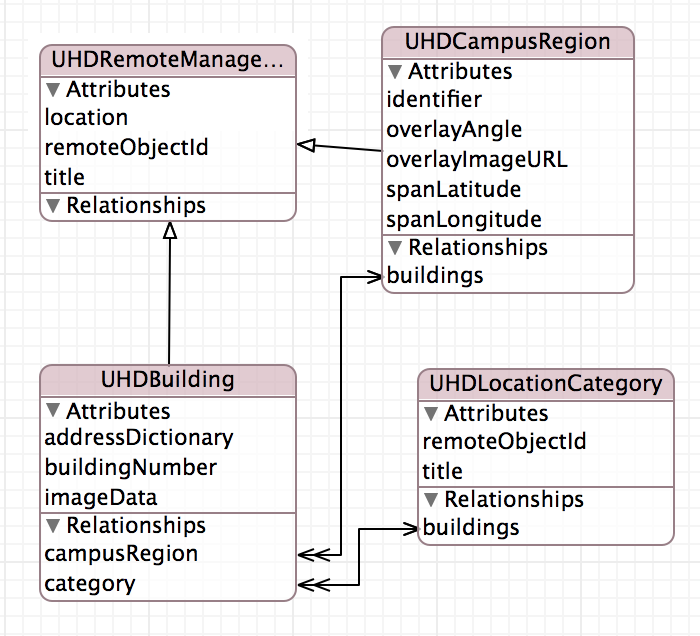
\includegraphics[scale=0.6]{Bilder/DataModel.png}}
\caption{Data Model der Maps}
\end{figure}

Zunächst ist klar, dass Gebäude als eine eigenständige Klasse implementiert werden müssen. Da jedes Gebäude einen Ort zugewiesen bekommt, welcher in der Karte durch eine Annotation eingefügt wird, muss das \objc{MKAnnotation}-\emph{Protokoll} implementiert werden. Dazu wird die Klasse \objc{UHDRemoteManagedLocation} erstellt. Diese ordnet jedem Gebäude verschiedene Eigenschaften, wie eben den Ort, aber auch einen \emph{Titel} und eine \emph{Kategorie} aus der später erläuterten Klasse \objc{UHDLocationCategory} zu. Die Gebäude selbst werden in der Klasse \objc{UHDBuilding} implementiert, welche zusätlich jedem Gebäude zusätzlich ein Bild und eine \objc{campusRegion} zuweist. Weiterhin wird jedem Objekt der Klasse ein \objc{identifier} übergeben, welcher den Titel richtig zusammensetzt. Dies ist darin begründet, dass beispielsweise Gebäude im Neuenheimer Feld alle den Zusatz \emph{INF} tragen, sodass dem Gebäude nur eine \objc{buildingNumber} zugeordnet werden muss. Der eigentliche \objc{title} des Gebäudes setzt sich dann aus beiden Teilen zusammen, was aufgrund der überschriebenen Getter-Methode des Identifiers geschieht:

\begin{objclst}
- (NSString *)identifier {
    return [NSString stringWithFormat:@"%@ %@", self.campusRegion.identifier, self.buildingNumber];
}
\end{objclst}

\noindent Um eine solche Charakterisierung der Gebäude zu erhalten, muss jedem Gebäude eine Region in Heidelberg zugeordnet werden. Dafür wird eine weitere Klasse \objc{UHDCampusRegion} erstellt, die es ermöglicht jedem Gebäude eine solche \objc{campusRegion} zuzuornden. Auch jede \objc{campusRegion} hat einen eigenen Identifier, welcher in der oben beschriebenen Getter-Methode für den Identifier der \objc{UHDBuilding}-\emph{Klasse} zu einem zusammengesetzten String übergeben wird. Damit erhält man also entweder mit dem Identifier \objc{INF} für das Neuenheimer Feld als eine \objc{campusRegion} und einer Gebäudenummer, z.B. \objc{227}, den \objc{building.indetifier} \objc{INF 227} oder im Falle der Altstadt mit dem Identifier \objc{Altstadt} den gleichen Identifier für das Gebäude selbst. Durch einen \objc{NSMutableSet} können einer \objc{campusRegion} mehrere Gebäude hinzugefügt werden. Die Klasse \objc{UHDCampusRegion} implementiert zudem das \objc{MKOverlay}-\emph{Protokoll}, welches später für die Kartenansicht im View interessant wird. Damit kann eigenes Kartenmaterial, wie die Lagekarten der Universität Heidelberg, über die eigentlich Map gelegt werden, um somit die Gebäude der Universiät hervorzuheben. Um weiterhin zwischen Gebäuden verschiedener Fakultäten oder auch Verwaltungsgebäuden zu unterscheiden, wird eine weitere Klasse \objc{UHDLocationCategory} erstellt, die jedem Objekt der Klasse \objc{UHDBuilding} eine \objc{category} zuordnet. Dadurch kann man beispielsweise im \objc{UHDMapsSearchTableViewController}, welcher in Abschnitt \ref{subsection_1} behandelt wird, speziell nach Gebäuden einer Fakultät suchen oder in der MapView sich nur Gebäude einer bestimmten Kategorie ansehen. 

\subsection{Implementierungsdateien}

\subsubsection{UHDRemoteManagedLocation.h}

\lstinputlisting{Model/UHDRemoteManagedLocation.h}

\vspace{0,5cm}

\subsubsection{UHDRemoteManagedLocation.m}

\lstinputlisting{Model/UHDRemoteManagedLocation.m}

\vspace{0,5cm}

\subsubsection{UHDBuilding.h}

\lstinputlisting{Model/UHDBuilding.h}

\vspace{0,5cm}

\subsubsection{UHDBuilding.m}

\lstinputlisting{Model/UHDBuilding.m}
\newpage
\subsubsection{UHDCampusRegion.h}

\lstinputlisting{Model/UHDCampusRegion.h}

\vspace{0,5cm}

\subsubsection{UHDCampusRegion.m}
\lstinputlisting{Model/UHDCampusRegion.m}

\vspace{0,5cm}

\subsubsection{UHDLocationCategory.h}
\lstinputlisting{Model/UHDLocationCategory.h}

\vspace{0,5cm}

\subsubsection{UHDLocationCategory.m}
\lstinputlisting{Model/UHDLocationCategory.m}

\newpage

\section{Darstellung der verschiedenen Views}

\begin{figure}[ht]\label{bild_2}
\centering \rotatebox{0}{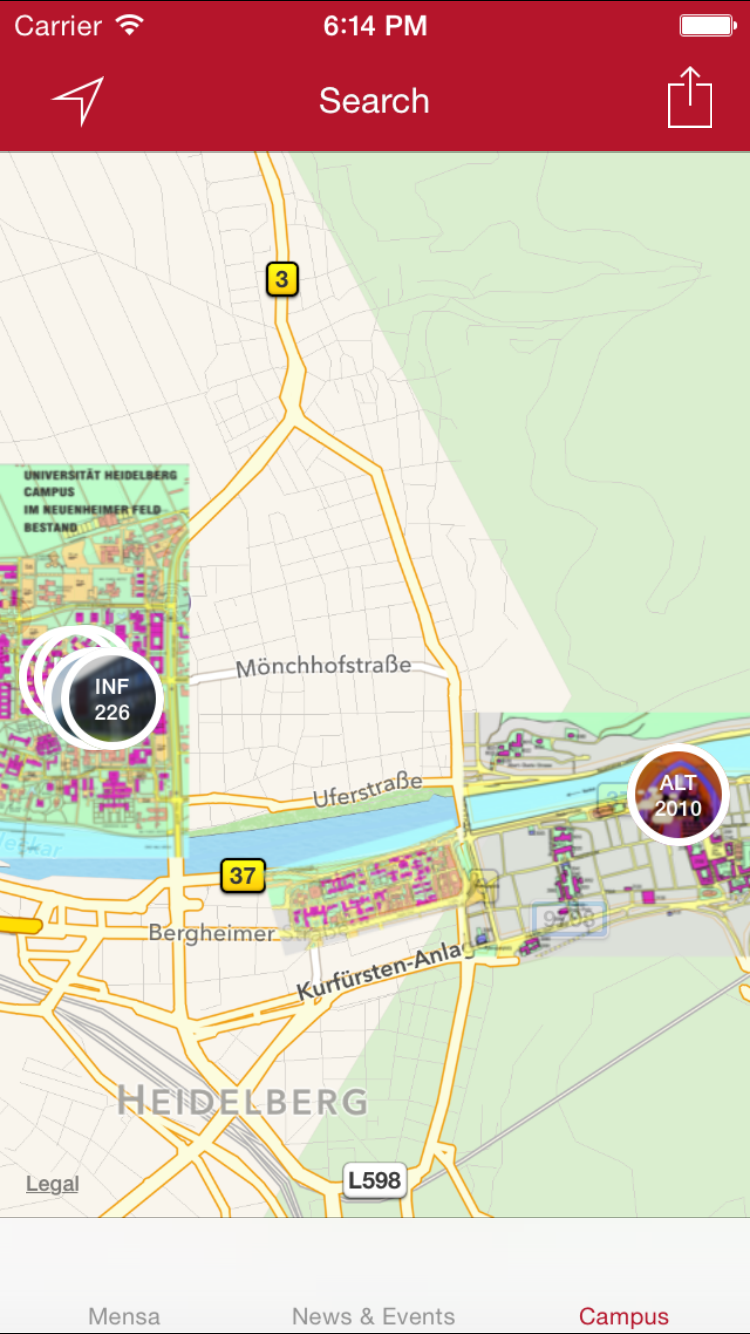
\includegraphics[scale=0.15]{Bilder/Bild_1.png}}
\caption{Ansicht der MapView nach Auswahl des \objc{Campus}-Buttons}
\end{figure}

Im \objc{NavigationViewController} kann über den Button \objc{Campus} die Anzeige der \objc{MKMapView} erreicht werden. Dort gibt es zunächst die Option die Karte in verschiedenen Ansichten darzustellen. Es gibt die Wahl zwischen \objc{Standard}, was die Standardarstellung der Karte in iOS ist, \objc{Hybrid} oder \objc{Satellite}. In der Klasse \objc{UHDBuildingAnnotationView} werden die Annotations angepasst, das heißt zum einen wird das Auftreten in der Map View durch ein Symbol und die Darstellung der Annotation selbst, beispielsweise mit Bild des Gebäudes oder einem Info-Button zur Weiterleitung auf den \objc{UHDBuildingDetailViewController}, bearbeitet. Die einzelnen Gebäude der Universität werden durch solche Symbole dargestellt \textbf{WELCHE SYMBOLE? BESCHREIBEN? BILD?????}. 

\begin{figure}[ht]\label{bild_3}
\centering \rotatebox{0}{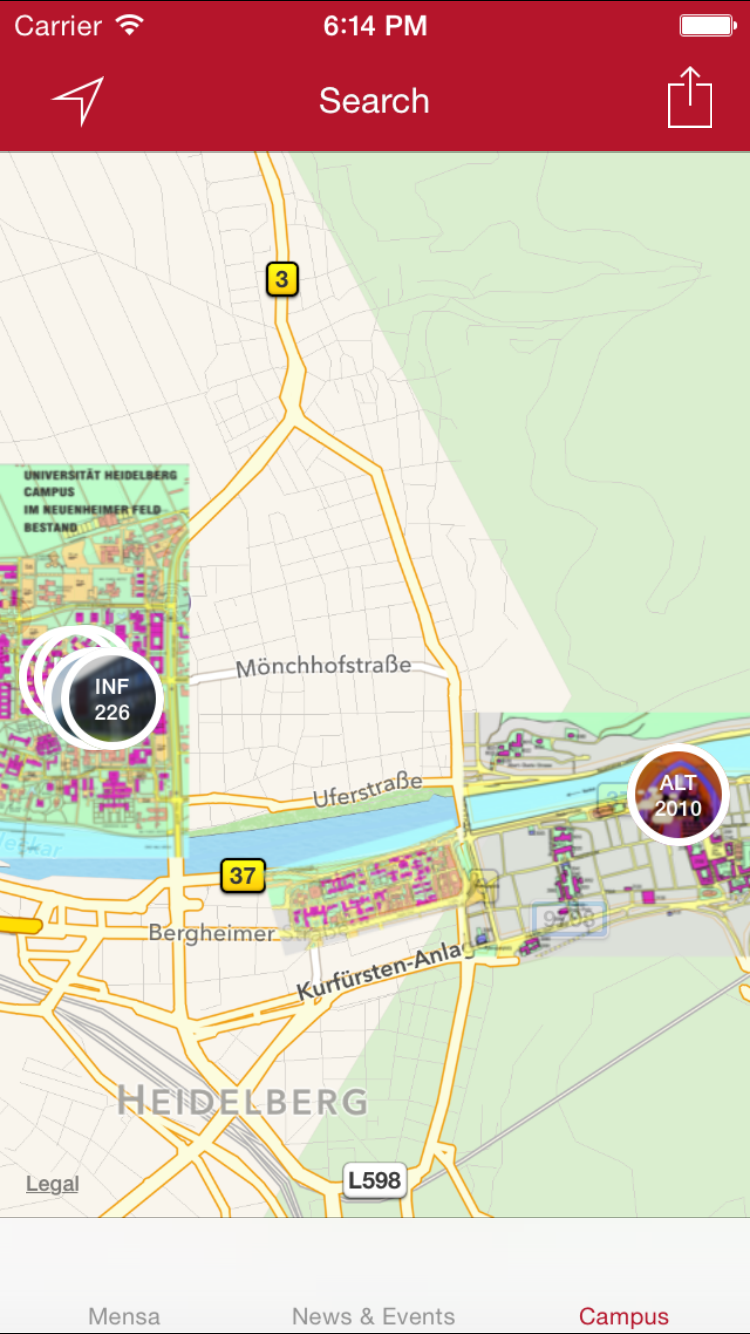
\includegraphics[scale=0.15]{Bilder/Bild_1.png}}
\caption{BILDERSATZ: BILD MIT SYMBOLEN UND UHDBuildingDetailView}
\end{figure}

Durch die Auswahl eines solchen Symbols erhält man zunächst grundlegende Informationen, wie den Titel und die Campus-Zugehörigkeit, in einer Art Sprechblase angezeigt. Das Tappen auf den Info-Button in dieser Sprechblase öffnet ein neues Fenester, welches alle Informationen zum Gebäude anzeigt. Diese Darstellung wird durch den \objc{UHDBuildingDetailViewController} implementiert. Zu den von Apple bereitgestellten Kartenansichten, lässt sich die MapView, wie bereits im vorherigen Kapitel angesprochen, durch ein sogenanntes Overlay modifizieren. Diese Kartendarstellung ist ein wenig aufwendiger zu implementieren, denn diese ist keine von Apple vorgefertigte Anzeigeoption. Stattdessen wurde dazu aus verschiedenen Lagekarten der Universität im PDF-Format, welches die Gebäude in verschiedenen Farben und mit Namen anzeigt, benutzt, um ein solches \emph{Overlay} zu erzeugen. Das heißt über die \objc{MapView} wurde das PDF gelegt und dort die Mitte mit der Property \objc{coordinate} bestehend aus \objc{centerLatitude} und \objc{centerLongitude} (siehe \objc{UHDCampusRegion.m}) als Fixpunkt gewählt. Durch Bestimmung der Breite \objc{deltaLongitude} und der Höhe \objc{deltaLatitude} des PDFs in geographischen Koordinaten konnte das \objc{boundingMapRect} konfiguriert werden und dadurch die genaue Position des Overlays eingestellt werden. 

\begin{figure}[ht]\label{bild_4}
\centering \rotatebox{0}{\includegraphics[scale=0.45]{Bilder/Bild_2.1.png}}
\caption{Overlay anhand des Beispiels Neuenheimer Feld (Der Pin stellt die Mitte dar)}
\end{figure}

Wir haben uns für diese zusätzliche Darstellung entschieden, da sie dem Benutzer einen viel besseren Überblick über die Gebäude der Universität liefert, als die eigentliche Karte in iOS. Um das Overlay korrekt darzustellen, wurde die Klasse \objc{UHDCampusRegionRender} implementiert, in der das Overlayimage dem View übergeben wird und durch die Methode \objc{- (void)drawMapRect: zoomScale: inContext:} in die jeweilige Region der MapView gelegt wird. {\red Weiterhin haben wir uns gedacht, dass der Nutzer am besten selbst entscheiden sollte, ob er das Overlay benutzen möchte oder nicht. Dazu befindet sich in Bild \ref{bild_4} oben links ein Button, durch den ein Slide von unten hineinkommt und dem Benutzer einige Einstellmöglichkeiten bietet. Hierbei wurde ein sogenannter \objc{Switch} eingefügt, mit dem das Overlay ein und ausgeschalten werden kann. Entscheidet sich also der Nutzer dazu, dass er die Map lieber ohne das Overlay benutzen möchte, dann kann er einfach immer diesen Schalter in der deaktivierende Position belassen. }

\begin{figure}[ht]\label{bild_5}
\centering \rotatebox{0}{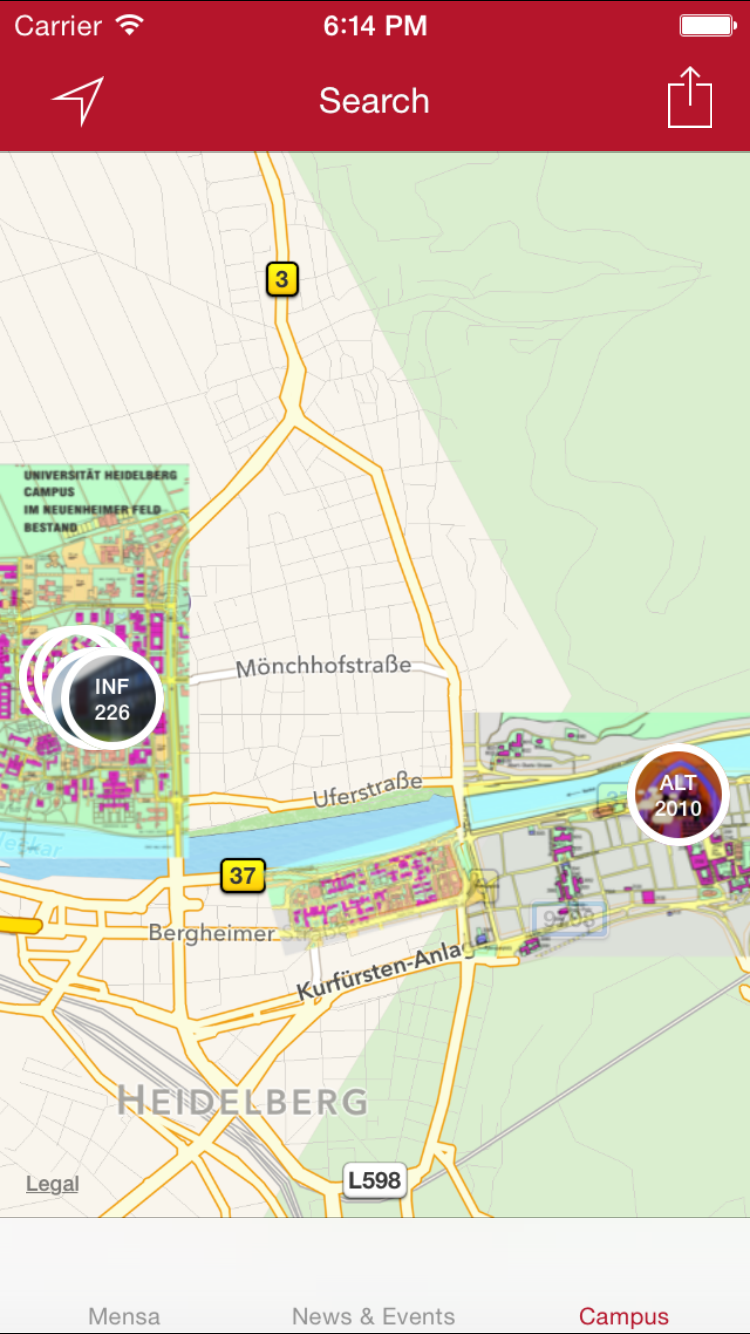
\includegraphics[scale=0.15]{Bilder/Bild_1.png}}
\caption{\textbf{BILD ZUR FUNKTIONSÜBERSICHT!!!!}}
\end{figure}

{\red \textbf{BESCHREIBUNG ZUR WEITEREN FUNKTIONSÜBERSICHT!!!}}

a

a

a

a

a

a

a

a

a

a


a


a


a

Drückt man in Bild \ref{bild_5} auf den oberen rechten Button mit dem Lupensymbol, so kommt man zunächst zum \objc{UHDMapsSearchTableViewController}, in dem einzelne Gebäude nach Kategorien geordnet dargestellt werden.

\begin{figure}[ht]\label{bild_6}
\centering \rotatebox{0}{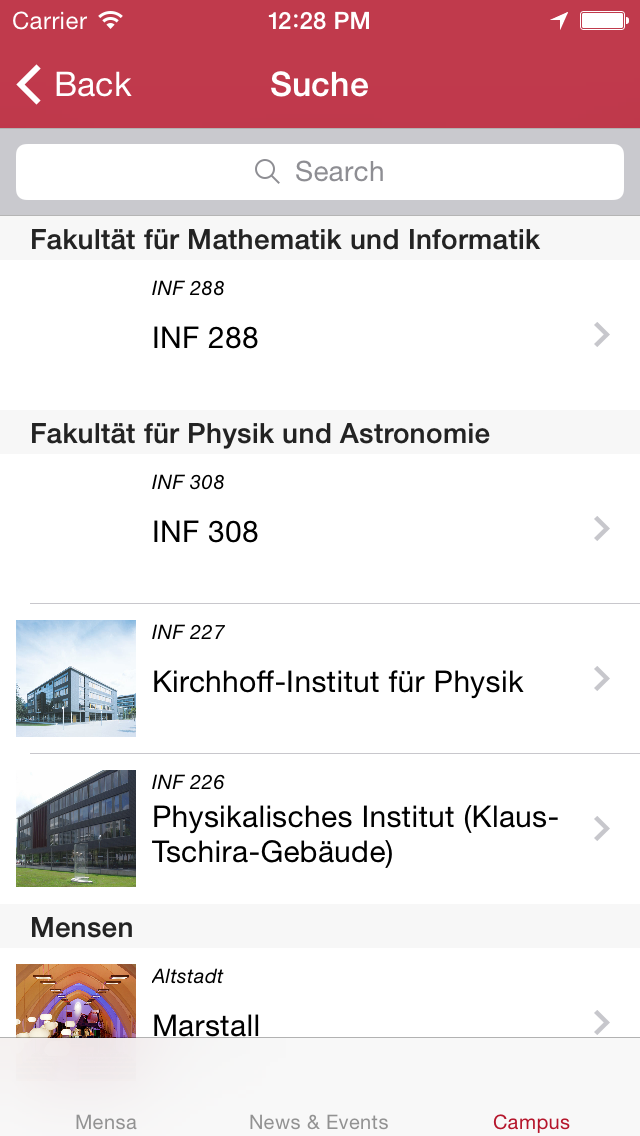
\includegraphics[scale=0.2]{Bilder/Bild_5.png}}
\caption{\objc{UHDMapsSearchTableViewController} mit Beispiel Daten}
\end{figure}

Dort wurde mit Hilfe einer \objc{UISearchBar} eine Suchfunktion integriert, bei dem nach bestimmten Gebäuden oder auch Gebäuden einer Fakultät gesucht werden kann. Zudem wurde die \objc{UITableView} in \objc{sections} unterteilt, welche die Gebäude einer Kategorie zusammenfasst. Mit einem Tap auf das gewünschte Gebäude kommt man auf die \objc{UHDBuildingDetailView}, wie sie in Bild \ref{bild_3} zu sehen ist. Dort sind alle Informationen über das Gebäude zusammengefasst dargestellt. Hier wird es vermutlich noch zu Erweiterungen hinsichtlich der angezeigten Daten kommen. Wir planen zudem Räume innerhalb der Gebäude, Professoren und Forschungsgruppen am jeweiligen Gebäude aufzulisten.

\section{Implementierung der View Controller}

\subsection{UHDMapsViewController}

\subsection{UHDBuildingDetailViewController}

\subsection{UHDMapsSearchTableViewController} \label{subsection_1}

\subsection{UHDMapsSearchCell+ConfigureForItem}


\newpage
\chapter{Zusammenfassung}

\end{document}